\documentclass{article}

% Language setting
% Replace `english' with e.g. `spanish' to change the document language
\usepackage[english]{babel}

% Set page size and margins
% Replace `letterpaper' with`a4paper' for UK/EU standard size
\usepackage[letterpaper,top=2cm,bottom=2cm,left=3cm,right=3cm,marginparwidth=1.75cm]{geometry}

% Useful packages
\usepackage{amsmath}
\usepackage{graphicx}
\usepackage[colorlinks=true, allcolors=blue]{hyperref}

\title{Cash-flow maturity and risk premia in CDS markets.}
\author{Antonio Pineda, Nidhi Beeravolu, Kausthub Keshava and Diana Castellanos}

\begin{document}
\maketitle

\begin{Data science tools for finance final project}
Professor: Jeremy Bejerano.
\end{abstract}

\section{Introduction}

The present project is an academic exercise designed to replicate and analyze the Credit Default Swap (CDS) returns specified by \cite{kelly2017}. The dataset, sourced from the repositories of Markit on Wharthon Research Data Services (WRDS), provides the data foundation upon which our replication model is constructed. \\

This work is designed to not only corroborate the meticulous work of \cite{kelly2017} but also to substantiate the theoretical implications proposed by \cite{Palhares2013} concerning the maturation of cash-flows and their correlation with the risk premia observed in the market for credit default swaps.\\

The paper is structured as follows. Section 2 introduces the model of CDS returns, detailing the theoretical framework and the mathematical underpinnings that guide the analysis. Section 3 provides a description of the data sourced from Markit and presents summary statistics to offer insights into the dataset's characteristics and the underlying market dynamics. Section 4 delves into the estimated CDS returns, employing the proposed model to analyze the dataset and interpret the results. The findings reveal that [WRITE RESULTS], highlighting the implications of [WRITE KEY VARIABLES] on CDS returns.  In conclusion, the paper demonstrates [WRITE MAIN CONCLUSION].


\section{Credit default swap returns definition.}

According to  \cite{Palhares2013}, CDS returns are definite as:

\begin{equation}
    CDS_{t}^{ret} = \frac{CDS_{t-1}}{250} + \Delta CDS_{t} \times RD_{t-1}.

\end{equation}

The right-hand side of the equation is composed of two parts: the carry component and the capital gain return. \

The carry component reflects the return accrued from the seller’s receipt of insurance premium payments. The second term represents the capital gain return, which is calculated by multiplying the change in the credit default swap (CDS) spread by the lagged risky duration of the contract, denoted as \( RD_{t-1} \). This risky duration adjusts the future CDS spread received by the seller to its present value. When this value is multiplied by the change in spread, it estimates the logarithmic capital gain for the seller who is in a short position.\\

The risky duration for CDS of maturity $M$ years with quarterly premium payments is computed as


\begin{equation}
RD_t = \frac{1}{4} \sum_{j=1}^{4M} e^{-\frac{j\lambda}{4}} \cdot e^{-\frac{j(r_{\frac{j}{4}, t})}{4}},
\end{equation}




where:\


$e^{-\frac{j\lambda}{4}}$ is the quarterly survival probability, \ 

$r^{\frac{j}{4}}_t$ is the risk-free rate for the quarter $\frac{j}{4}$,\

and $e^{-j\frac{j(r^{\frac{j}{4}})}_{4}}$ is the quarterly discount function. And  $\lambda$ each day from the 5-year spread as

\[
\lambda = 4 \log \left(1 + \frac{\text{CDS}}{4L}\right),
\]

where $\text{CDS}$ is the spread and $L$ is the loss given default (assumed to be 60\%). The risk-free term structure is constructed using swap rates for maturities 3 and 6 months and US Treasury yields for maturities from 1 year to 10 years.


\section{Data.}
In this section, We first describe the data sources that we use and give an overview of the data. Then how we calculated CDS returns


We utilized the Par Spread data corresponding to a five-year tenor sourced from CRSP, spanning the years 2001 to 2004, for our analysis of Credit Default Swap (CDS) spreads. This dataset encompassed all available tickers, which we then categorized into quantiles. Subsequently, we arranged these quantiles to form 20 distinct portfolios sequentially. Additionally, we applied a smoothing technique specifically to the portfolio corresponding to the 20th quantile. 

%insert graphs
%![Image Description](../assets/cds_box_plot.png)

\begin{figure}[H]
    \centering
    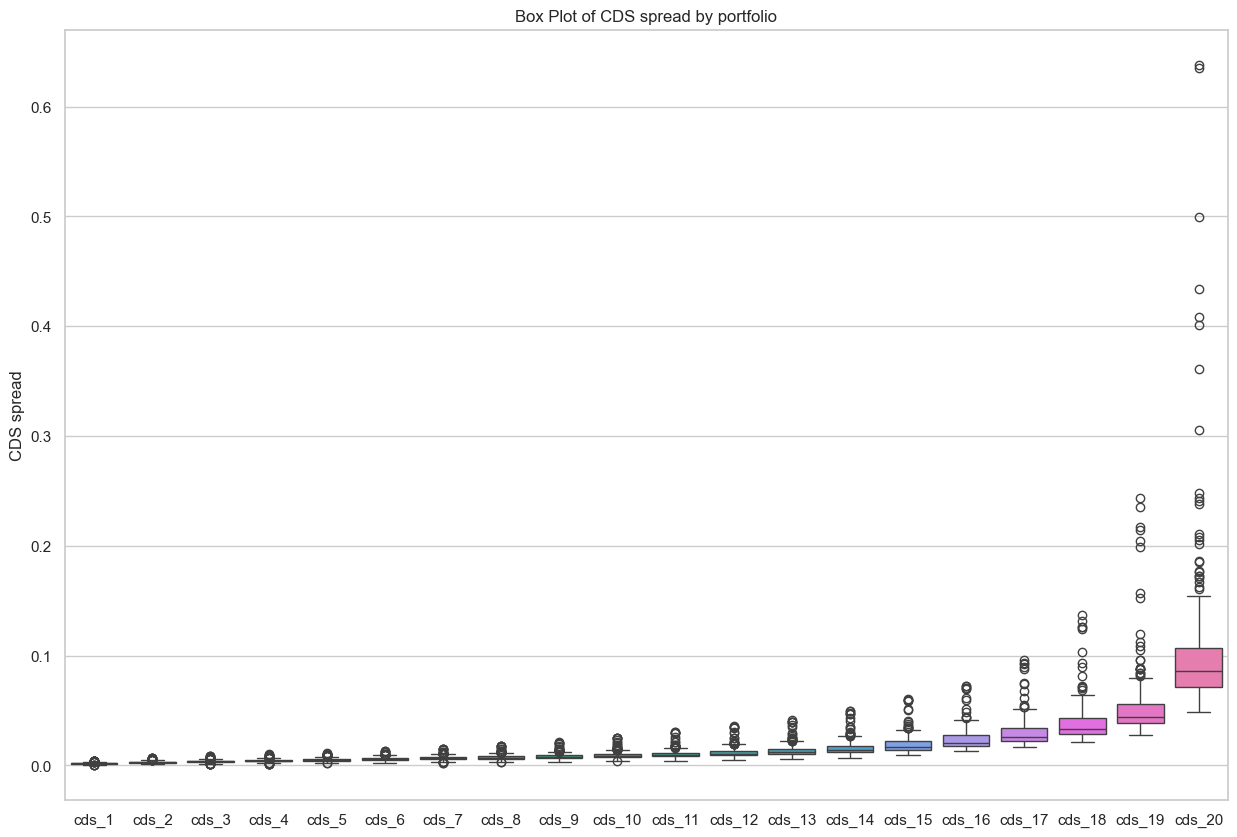
\includegraphics[width=0.75\textwidth]{../assets/cds_box_plot.png}
    \caption{\label{fig:myplot}Box plot of CDS returns across 20 portfolios.}
    \end{figure}

For rates of 3-6 months we used Fred website and for rates of 1-10 years, FED website and filtered by the date of the CDS data. We used the rates for maturities 3 and 6 months and US Treasury yields for maturities from 1 year to 10 years and extrapolated it to construct the risk-free term structure.

% WRITE ABOUT THE EXTRAPOLATION OF THE RATES

\begin{figure}[H]
    \centering
    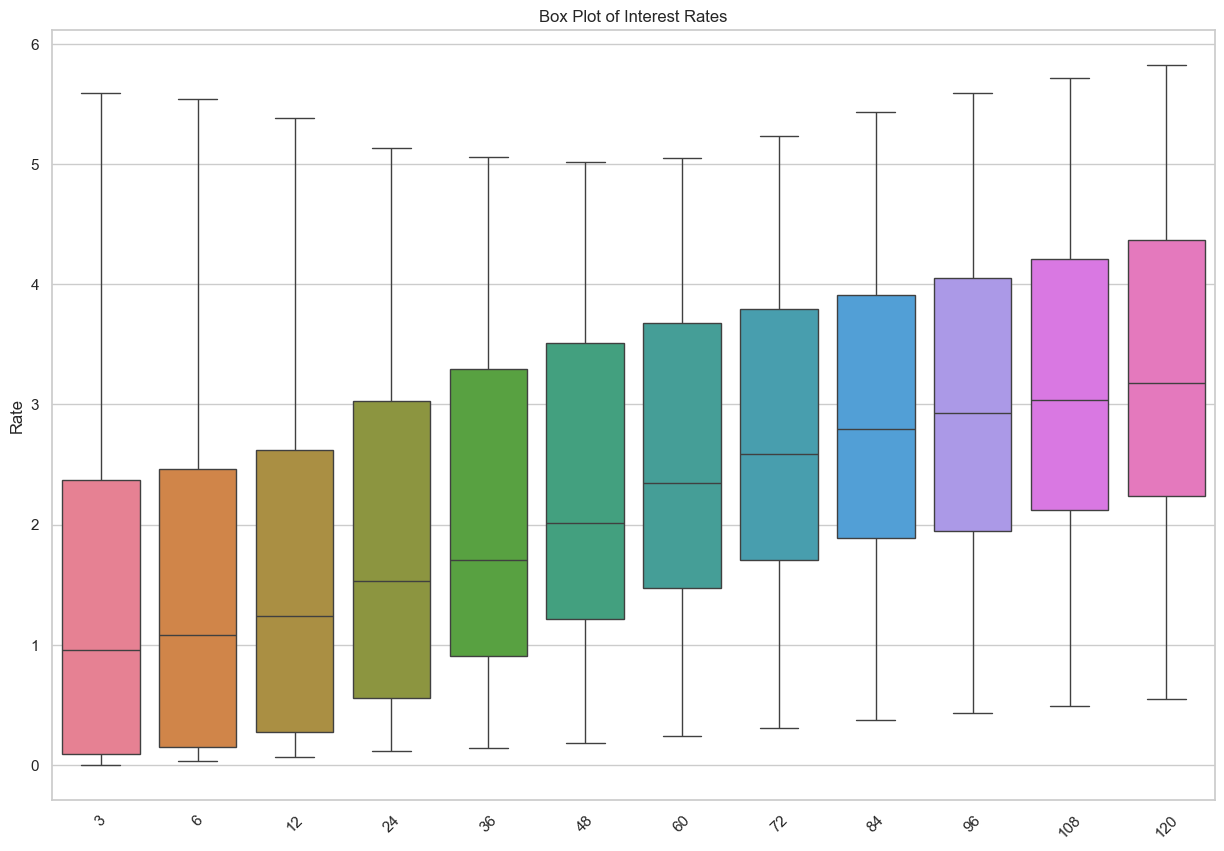
\includegraphics[width=0.75\textwidth]{../assets/rates_boxplot.png}
    \caption{\label{fig:myplot}Box plot of CDS rates from 3 to 120 monts (10 years).}
    \end{figure}

\begin{figure}[H]
    \centering
    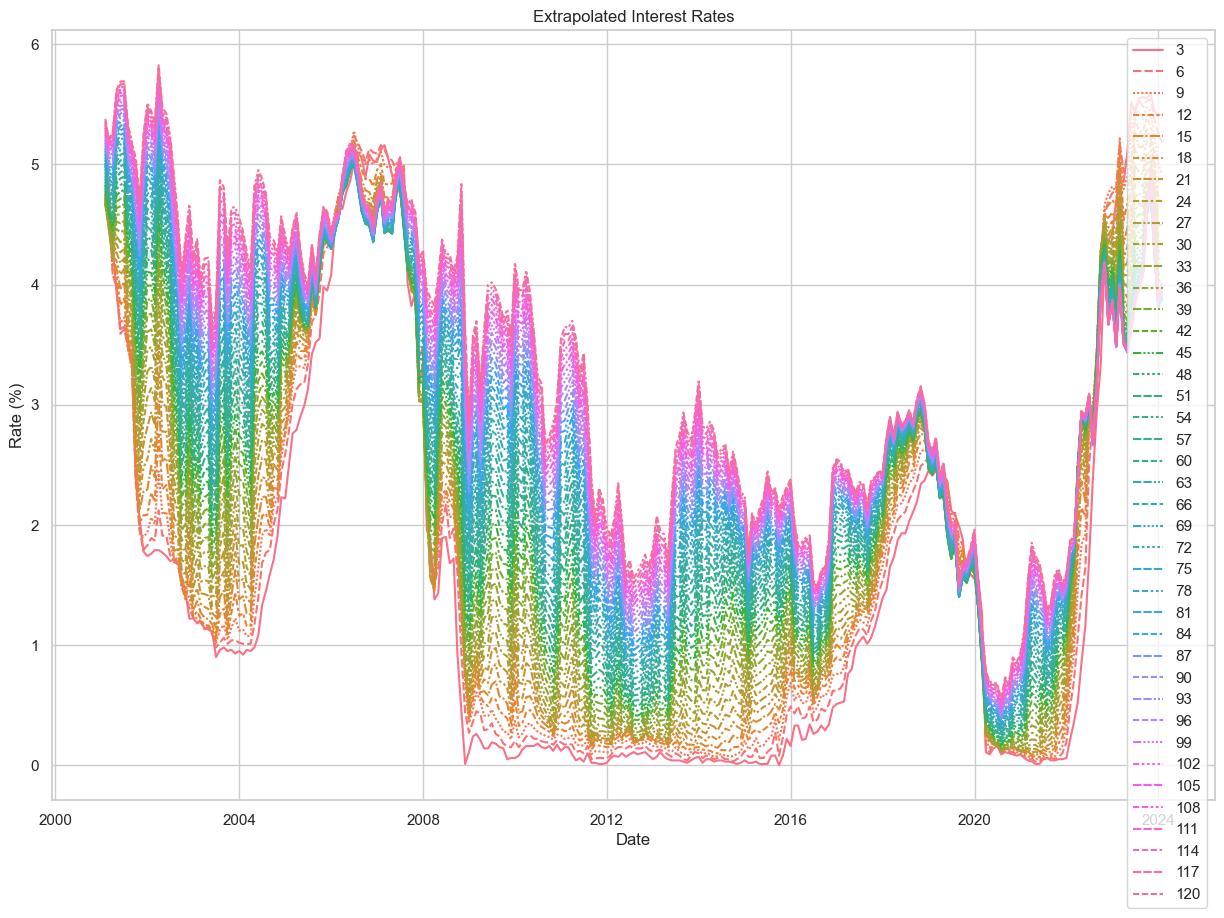
\includegraphics[width=0.75\textwidth]{../assets/extrapolated_interest_Rates.png}
    \caption{\label{fig:myplot}Extrapolated interest rates.}
    \end{figure}    


\section{Results.}

% ADD RESULTS AND GRAPHS, CHECK IF THE NEGATIVE RELATION IS TRUE OR ADD SOME CONCLUSION


\bibliographystyle{alpha}
\bibliography{bibliography}

\end{document}